\documentclass[reqno]{amsart}
\usepackage{amscd, amssymb, amsmath, amsthm}
\usepackage{graphicx}
\usepackage[colorlinks=true,linkcolor=blue]{hyperref}
\usepackage[utf8]{inputenc}
\usepackage[T1]{fontenc}
\usepackage{textcomp}
\usepackage{babel}
%% for identity function 1:
\usepackage{bbm}
%%For category theory diagrams:
\usepackage{tikz-cd}


\setlength\parindent{0pt}

\pdfsuppresswarningpagegroup=1

\newtheorem{theorem}{Theorem}[section]
\newtheorem{lemma}[theorem]{Lemma}
\newtheorem{proposition}[theorem]{Proposition}
\newtheorem{corollary}[theorem]{Corollary}
\newtheorem{conjecture}[theorem]{Conjecture}

\theoremstyle{definition}
\newtheorem{definition}[theorem]{Definition}
\newtheorem{example}[theorem]{Example}
\newtheorem{exercise}[theorem]{Exercise}
\newtheorem{problem}[theorem]{Problem}
\newtheorem{question}[theorem]{Question}

\theoremstyle{remark}
\newtheorem*{remark}{Remark}
\newtheorem*{note}{Note}
\newtheorem*{solution}{Solution}



%Inequalities
\newcommand{\cycsum}{\sum_{\mathrm{cyc}}}
\newcommand{\symsum}{\sum_{\mathrm{sym}}}
\newcommand{\cycprod}{\prod_{\mathrm{cyc}}}
\newcommand{\symprod}{\prod_{\mathrm{sym}}}

%Linear Algebra

\DeclareMathOperator{\Span}{span}
\DeclareMathOperator{\im}{im}
\DeclareMathOperator{\diag}{diag}
\DeclareMathOperator{\Ker}{Ker}
\DeclareMathOperator{\ob}{ob}
\DeclareMathOperator{\Hom}{Hom}
\DeclareMathOperator{\Mor}{Mor}
\DeclareMathOperator{\sk}{sk}
\DeclareMathOperator{\Vect}{Vect}
\DeclareMathOperator{\Set}{Set}
\DeclareMathOperator{\Group}{Group}
\DeclareMathOperator{\Ring}{Ring}
\DeclareMathOperator{\Ab}{Ab}
\DeclareMathOperator{\Top}{Top}
\DeclareMathOperator{\hTop}{hTop}
\DeclareMathOperator{\Htpy}{Htpy}
\DeclareMathOperator{\Cat}{Cat}
\DeclareMathOperator{\CAT}{CAT}
\DeclareMathOperator{\Cone}{Cone}
\DeclareMathOperator{\dom}{dom}
\DeclareMathOperator{\cod}{cod}
\DeclareMathOperator{\Aut}{Aut}
\DeclareMathOperator{\Mat}{Mat}
\DeclareMathOperator{\Fin}{Fin}
\DeclareMathOperator{\rel}{rel}
\DeclareMathOperator{\Int}{Int}
\DeclareMathOperator{\sgn}{sgn}
\DeclareMathOperator{\Homeo}{Homeo}
\DeclareMathOperator{\SHomeo}{SHomeo}
\DeclareMathOperator{\PSL}{PSL}
\DeclareMathOperator{\Bil}{Bil}
\DeclareMathOperator{\Sym}{Sym}
\DeclareMathOperator{\Skew}{Skew}
\DeclareMathOperator{\Alt}{Alt}
\DeclareMathOperator{\Quad}{Quad}
\DeclareMathOperator{\Sin}{Sin}
\DeclareMathOperator{\Supp}{Supp}
\DeclareMathOperator{\Teich}{Teich}
\DeclareMathOperator{\tr}{tr}


%Row operations
\newcommand{\elem}[1]{% elementary operations
\xrightarrow{\substack{#1}}%
}

\newcommand{\lelem}[1]{% elementary operations (left alignment)
\xrightarrow{\begin{subarray}{l}#1\end{subarray}}%
}

%SS
\DeclareMathOperator{\supp}{supp}
\DeclareMathOperator{\Var}{Var}

%NT
\DeclareMathOperator{\ord}{ord}

%Alg
\DeclareMathOperator{\Rad}{Rad}
\DeclareMathOperator{\Jac}{Jac}

%Misc
\newcommand{\SL}{{\mathrm{SL}}}
\newcommand{\mobgp}{{\mathrm{PSL}_2(\mathbb{C})}}
\newcommand{\id}{{\mathrm{id}}}
\newcommand{\Mod}{{\mathrm{Mod}}}
\newcommand{\PMod}{{\mathrm{PMod}}}
\newcommand{\SMod}{{\mathrm{SMod}}}
\newcommand{\ud}{{\mathrm{d}}}
\newcommand{\Vol}{{\mathrm{Vol}}}
\newcommand{\Area}{{\mathrm{Area}}}
\newcommand{\diam}{{\mathrm{diam}}}
\newcommand{\End}{{\mathrm{End}}}


\newcommand{\reg}{{\mathtt{reg}}}
\newcommand{\geo}{{\mathtt{geo}}}

\newcommand{\tori}{{\mathcal{T}}}
\newcommand{\cpn}{{\mathtt{c}}}
\newcommand{\pat}{{\mathtt{p}}}

\let\Cap\undefined
\newcommand{\Cap}{{\mathcal{C}}ap}
\newcommand{\Push}{{\mathcal{P}}ush}
\newcommand{\Forget}{{\mathcal{F}}orget}


\title{Notes on Isospectral Riemann Surfaces}
\author{Jonas Trepiakas}
\date{}

\begin{document}
\maketitle

We will follow the text 'Isospectral Riemann Surfaces' by Peter Buser.


\section{Pasting}\label{sec:pasting}
We will have two pasting constructions which will give
us two different surfaces. They will both be made up of 
eight hyperbolic octagons glued together as shown in
Figure \ref{octagon-gluing-png}.

\begin{figure}[htpb]
    \centering
    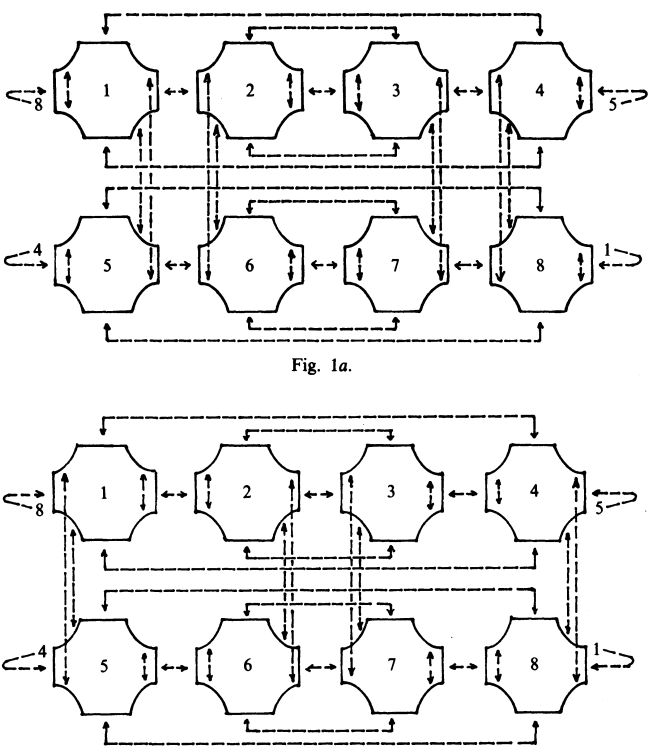
\includegraphics[width=0.6\textwidth]{octagon-gluing.png}
    \caption{octagon-gluing.png}
    \label{fig:octagon-gluing-png}
\end{figure}

\subsection{Genus five}

For a pentagon with sides $r,p,q,q',p'$, the following
trigonometric formulae hold
\begin{align*}
    \cosh r &= \coth p \coth p'\\
    \cosh r &= \sinh q \sinh q'.
\end{align*}
Moreover, such pentagons exist for any $q',r \in \mathbb{R}_{>0}$.

Consequently, for any length of the sides
$b'$ and $c'$ in Figure \ref{fig:hyperbolic-octagon-png} 
we can construct such an octagon.
By construction,
$a' = a'' = a^{*} = a^{* *}$ and $ c'=c''$, so
the pasting of section \ref{sec:pasting} is possible.


\begin{figure}[htpb]
    \centering
    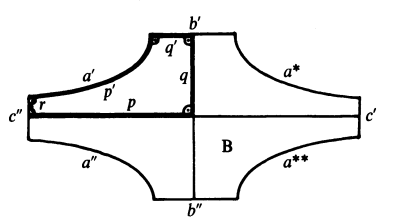
\includegraphics[width=0.5\textwidth]{hyperbolic-octagon.png}
    \caption{hyperbolic-octagon.png}
    \label{fig:hyperbolic-octagon-png}
\end{figure}


\begin{lemma}[]\label{lemma3.3}
    Let $0 < c' < b' <1$. Then any curve $\delta$ on
    $B$ which connects two non adjacent sides of $B$ has
    length $\ell \left( \delta \right) \ge c'$. Equality
    holds for $\delta = c'$ and $\delta = c''$.
\end{lemma}

\begin{proof}
    Recall that with negative curvature, the unique shortest
    connecting curve $\delta$ between two non intersecting
    geodesics is the common perpendicular between these
    geodesics. Now
    $\sinh q \sinh q' = \cosh r > 1$ and
    $q' = \frac{1}{2} b' < 1$ together imply $q > 1$. Similarly,
    $p',p >  1$. It follows from Figure
    \ref{fig:hyperbolic-octagon-png} that
    if  $\delta$ is not $c'$ or $c''$ then
    it has length $\ell (\delta) > c' = c''$.
\end{proof}

\begin{proposition}[]
    Under the hypothesis of Lemma \ref{lemma3.3},
    $S_1$ and $S_2$ are non isometric.
\end{proposition}

\subsection{The length spectrum}

\begin{definition}[Length Spectrum]
    For a compact Riemannian manifold we define
    the \textit{length spectrum} to be the function
    $\ell \mapsto  n_M(\ell)$ which associates
    to each positive real number $\ell$ the cardinality
    $n_M\left( \ell  \right) $ of the set of all
    closed geodesics of length $\ell $ on $M$.
\end{definition}

\begin{corollary}
    Recall that for a compact Riemann surface of genus
    $g\ge 2$, each free homotopy class of an essential
    closed curve, there is a unique closed geodesic.
    Hence the number of closed geodesics of length
    $\le \ell $ is finite for all $\ell$. The
    length spectrum here may also be defined by giving
    the list of all possible lengths, arranged in
    increasing order.
\end{corollary}

\begin{theorem}[]
    Two compact Riemann surfaces of genus
    $g\ge 2$ are isospectral with respect to the
    Laplacian if and only if they have the same
    length spectrum. 
\end{theorem}

\begin{proposition}[]
    The surfaces $S_1$ and $S_2$ obtained in
    section \ref{sec:pasting} have the same length spectrum.
\end{proposition}






    %\bibliography{../refs.bib}
\end{document}
